% !TeX program = xelatex
\ifdefined\BookMaster\else
\documentclass[11pt,oneside]{article}
% !TeX program = xelatex
\usepackage[b5paper,left=22mm,right=22mm,top=20mm,bottom=22mm,footskip=11mm]{geometry}
\usepackage{fontspec}
\setmainfont{TeX Gyre Termes}
\setsansfont{TeX Gyre Heros}
\usepackage{amsmath,amssymb,mathtools,amsthm}
\renewcommand{\cdots}{\mathinner{\cdotp\cdotp\cdotp}}
\usepackage{graphicx,adjustbox,array,booktabs,longtable,multirow,enumitem,changepage,needspace}
\usepackage[table]{xcolor}
\usepackage{fancyhdr}
\raggedbottom
\interfootnotelinepenalty=10000
\newcommand{\BookFootnote}[2]{\begingroup\renewcommand{\thefootnote}{\fnsymbol{footnote}}\footnote[#1]{#2}\endgroup}
\newcommand{\BookFootnoteMark}[1]{\begingroup\renewcommand{\thefootnote}{\fnsymbol{footnote}}\footnotemark[#1]\endgroup}
\newcommand{\BookFootnoteText}[2]{\begingroup\renewcommand{\thefootnote}{\fnsymbol{footnote}}\footnotetext[#1]{#2}\endgroup}
\newenvironment{BookFloat}[1]{\par\addvspace{.6\baselineskip}\noindent\def\BookFloatID{#1}\begin{minipage}{\linewidth}\phantomsection\label{bookfloat:#1:start}}{\phantomsection\label{bookfloat:\BookFloatID:end}\end{minipage}\par\addvspace{.6\baselineskip}}

\usepackage[unicode,hidelinks]{hyperref}
\pagestyle{fancy}
\fancyhf{}
\newcommand{\BookFooter}{}
\fancyfoot[L]{\parbox[b]{\dimexpr\textwidth-15mm}{\footnotesize\BookFooter}}
\fancyfoot[R]{\footnotesize\thepage}
\renewcommand{\headrulewidth}{0pt}
\renewcommand{\footrulewidth}{0pt}
\setlength{\parindent}{0pt}
\setlength{\parskip}{0.2em}
\setlength{\emergencystretch}{3em}
\setlist{nosep,leftmargin=1.7em,labelsep=.65em}
\newif\ifBookNarrative
\BookNarrativetrue
\newenvironment{BookBody}{\setlength{\parindent}{0pt}}{}
\newcommand{\BookStatement}[1]{\par\addvspace{.6\baselineskip}\noindent #1\enspace\ignorespaces}
\newcommand{\BookLabel}[1]{\par\addvspace{.6\baselineskip}\needspace{3\baselineskip}\noindent\textbf{#1}\quad\ignorespaces}
\newcommand{\BookHeading}[1]{\par\addvspace{\baselineskip}\needspace{4\baselineskip}\noindent{\large\bfseries #1}\par\medskip}
\newcommand{\BookSubheading}[1]{\par\addvspace{.7\baselineskip}\needspace{3\baselineskip}\noindent{\bfseries #1}\par\smallskip}
\newcommand{\BookTextHeading}[1]{\par\addvspace{.7\baselineskip}\needspace{3\baselineskip}\noindent #1\par\smallskip}
\newcommand{\BookSectionTitle}[2]{\par\addvspace{1.2\baselineskip}\needspace{5\baselineskip}\noindent\colorbox{gray!25}{\sffamily\bfseries\small SECTION #1}\quad{\large\bfseries #2}\par\medskip}
\newcommand{\BookExerciseTitle}[1]{\par\addvspace{\baselineskip}\needspace{4\baselineskip}\noindent{\color{gray}\rule{1.5mm}{1.5mm}}\enspace{\large\bfseries Exercises #1}\par\medskip}
\newcommand{\BookBullet}[1]{\begin{list}{\textbullet}{\setlength{\leftmargin}{1.7em}\setlength{\labelwidth}{1em}\setlength{\labelsep}{.7em}\setlength{\topsep}{0pt}\setlength{\parsep}{0pt}\setlength{\itemsep}{0pt}}\item #1\end{list}}
\newcommand{\BookExercise}[2]{\begin{list}{\textbf{#1}}{\setlength{\leftmargin}{2.2em}\setlength{\labelwidth}{1.5em}\setlength{\labelsep}{.7em}\setlength{\topsep}{.15em}\setlength{\parsep}{0pt}\setlength{\itemsep}{0pt}}\item #2\end{list}}
\newcommand{\BookEnd}[1]{\unskip\nobreak\hfill\ensuremath{#1}}
\newcommand{\BookSource}[2]{\phantomsection\label{sourcepage:#1}} % Source-page anchors, retained through reflow.
\usepackage{multicol}
\usepackage{tikz}
\newcommand{\BookPartEntry}[2]{\par\noindent\makebox[17mm][l]{\bfseries Section #1}#2\par}
\newcommand{\BookPartTitle}[3]{\par\bigskip\noindent\begin{tikzpicture}\node[anchor=north west,inner sep=0pt,outer sep=0pt] (bookpart) at (0,0) {\begin{minipage}{\dimexpr\linewidth-.5pt}\hspace*{26mm}\begin{minipage}[t]{\dimexpr\linewidth-26mm}\begin{adjustbox}{max width=\linewidth}{\fontsize{20}{24}\selectfont\bfseries #2}\end{adjustbox}\par\vspace{6mm}\hrule\vspace{6mm}{\sffamily\footnotesize\setlength{\parskip}{.3em}#3}\vspace{3mm}\end{minipage}\end{minipage}};\path[shade,top color=gray!60,bottom color=white] (0,0) rectangle ([xshift=24mm]bookpart.south west);\node[anchor=north,font=\sffamily\bfseries\small] at (12mm,-2mm) {PART};\node[anchor=north,font=\sffamily\bfseries\Huge] at (12mm,-7mm) {#1};\end{tikzpicture}\par\bigskip}
\newsavebox{\BookMathBox}
\makeatletter
\newcommand{\BookInline}[1]{\leavevmode\hskip0pt\relax\begingroup\in@{\begin}{#1}\ifin@\sbox{\BookMathBox}{\(#1\)}\ifdim\wd\BookMathBox>\dimexpr\linewidth-1em\relax\resizebox{\dimexpr\linewidth-1em\relax}{!}{\usebox{\BookMathBox}}\else\(#1\)\fi\else\in@{\left}{#1}\ifin@\sbox{\BookMathBox}{\(#1\)}\ifdim\wd\BookMathBox>\dimexpr\linewidth-1em\relax\resizebox{\dimexpr\linewidth-1em\relax}{!}{\usebox{\BookMathBox}}\else\(#1\)\fi\else\(#1\)\fi\fi\endgroup\hskip0pt\relax}
\makeatother
\DeclareMathOperator{\Aut}{Aut}
\DeclareMathOperator{\End}{End}
\DeclareMathOperator{\Hom}{Hom}
\DeclareMathOperator{\GF}{GF}
\DeclareMathOperator{\irr}{irr}
\DeclareMathOperator{\lt}{lt}
\DeclareMathOperator{\lp}{lp}
\providecommand{\textcircled}[1]{\textnormal{(#1)}}

\begin{document}
\fi
\renewcommand{\BookFooter}{Section 8 Groups of Permutations}
\pdfbookmark[0]{Section 8 Groups of Permutations}{08_groups_of_permutations}
\ifdefined\BookMaster\else\setcounter{page}{77}\fi
% Source PDF page 94; original printed page 77
\BookSource{94}{77}
\BookPartTitle{II}{Structure of Groups}{\BookPartEntry{8}{Groups of Permutations}
\BookPartEntry{9}{Finitely Generated Abelian Groups}
\BookPartEntry{10}{Cosets and the Theorem of Lagrange}
\BookPartEntry{11}{Plane Isometries}}

\BookNarrativetrue

\begin{BookBody}

\BookSectionTitle{8}{Groups of Permutations}

\noindent Let \BookInline{\phi:G\to G^{\prime }} be a function mapping the group \BookInline{G} to \BookInline{G^{\prime }.} Recall that the homomorphism property of an isomorphism states that for all \BookInline{a,\allowbreak b\in G,\allowbreak \phi (ab)= \phi (a)\phi (b).} Whenever a function has this property whether or not the function is one-to-one or onto, we say that \BookInline{\phi } is a\textbf{ group homomorphism}. Of course any group isomorphism is a group homomorphism, but the reverse is not necessarily true.

\BookLabel{8.1 Definition} Let \BookInline{G} and \BookInline{G^{\prime }} be groups with \BookInline{\phi:G\to G^{\prime }.} The map \BookInline{\phi } is a\textbf{ homomorphism} if the homomorphism property

\begin{center}\begin{adjustbox}{max width=\linewidth}\BookInline{\displaystyle \phi (ab)= \phi (a)\phi (b)}\end{adjustbox}\end{center}

\noindent holds for all \BookInline{a,\allowbreak b\in G.} \BookEnd{\blacksquare}

\BookLabel{8.2 Example} Let \BookInline{\phi:\mathbb{R}\to U(}the circle group) be defined by the formula

\begin{center}\begin{adjustbox}{max width=\linewidth}\BookInline{\displaystyle \phi (x)= \;\text{cos}\;(2\pi x)+ i\;\text{sin}\;(2\pi x)= e^{2\pi ix}.}\end{adjustbox}\end{center}

\noindent Then

\begin{center}\begin{adjustbox}{max width=\linewidth}\BookInline{\displaystyle \phi (a+ b)= \;\text{cos}\;(2\pi (a+ b))+ i\;\text{sin}\;(2\pi (a+ b))= e^{2\pi i(a+ b)}.}\end{adjustbox}\end{center}

\noindent Using either the usual properties of the exponential function or the formulas from trigonometry involving the sum of two angles, we see that

\begin{center}\begin{adjustbox}{max width=\linewidth}\BookInline{\displaystyle \phi (a+ b)= (\;\text{cos}\;(2\pi a)+ i\;\text{sin}\;(2\pi a))(\;\text{cos}\;(2\pi b)+ i\;\text{sin}\;(2\pi b))= e^{2\pi ai}e^{2\pi bi},\allowbreak }\end{adjustbox}\end{center}

\noindent so

\begin{center}\begin{adjustbox}{max width=\linewidth}\BookInline{\displaystyle \phi (a+ b)= \phi (a)\phi (b),\allowbreak }\end{adjustbox}\end{center}

\noindent which says that \BookInline{\phi } is a group homomorphism. Although \BookInline{\phi } maps onto \BookInline{U,\allowbreak } it is not one-toone, so \BookInline{\phi } is not an isomorphism.

The identity \BookInline{0\in \mathbb{R}} maps to 1, the identity in \BookInline{U.} Furthermore, for any \BookInline{x\in \mathbb{R},\allowbreak }

\begin{center}\begin{adjustbox}{max width=\linewidth}\BookInline{\displaystyle \phi ( - x ) = e ^ { - 2 \pi i x } = { \frac { 1 } { e ^ { 2 \pi i x } } } = ( \phi ( x ) ) ^ { - 1 } .}\end{adjustbox}\end{center} \BookEnd{\blacktriangle}

\end{BookBody}

% Source PDF page 95; original printed page 78
\BookSource{95}{78}
\BookNarrativetrue

\begin{BookBody}

\BookLabel{8.3 Example} Recall that \BookInline{U_{n}= \{z\in \mathbb{C}\mid z^{n}= 1\}.} Let \BookInline{\phi:U_{28}\to U_{4}} be given by \BookInline{\phi (z)= z^{7}.} To check that \BookInline{\phi } is well defined, we see that if \BookInline{z\in U_{28},\allowbreak } then \BookInline{z^{28}= 1.} Therefore\BookInline{,\allowbreak (z^{7})^{4}= 1,\allowbreak } which implies that \BookInline{z^{7}\in U_{4}.} We check that \BookInline{\phi } is a homomorphism.

\begin{center}\begin{adjustbox}{max width=\linewidth}\BookInline{\displaystyle \phi (z_{1}z_{2})= (z_{1}z_{2})^{7}= z_{1}^{7}z_{2}^{7}= \phi (z_{1})\phi (z_{2}).}\end{adjustbox}\end{center}

\noindent As in the previous example\BookInline{,\allowbreak \phi } maps the identity in \BookInline{U_{28},\allowbreak } in this case 1, to the identity 1 in \BookInline{U_{4}.} Furthermore,

\begin{center}\begin{adjustbox}{max width=\linewidth}\BookInline{\displaystyle \phi (z^{- 1})= z^{- 7}= (z^{7})^{- 1}= (\phi (z))^{- 1}.}\end{adjustbox}\end{center} \BookEnd{\blacktriangle}

\BookLabel{8.4 Definition} Let \BookInline{\phi:X\to Y} and suppose that \BookInline{A\subseteq X} and \BookInline{B\subseteq Y.} The set \BookInline{\phi [A]= \{\phi (a)\mid a\in A\}} is called the\textbf{ image of} \BookInline{A} \textbf{in} \BookInline{Y} \textbf{under the mapping} \BookInline{\phi.} The set \BookInline{\phi ^{- 1}[B]= \{a\in A\mid \phi (a)\in B\}} is called the\textbf{ inverse image of} \BookInline{B} \textbf{under the mapping} \BookInline{\phi.}\BookEnd{\blacksquare}

\noindent The four properties of a homomorphism given in the theorem that follows are obvious in the case of an isomorphism since we think of an isomorphism as simply relabeling the elements of a group. However, it is not obvious that these properties hold for all homomorphisms whether or not they are one-to-one or onto maps. Consequently, we give careful proofs of all four properties.

\BookLabel{8.5 Theorem} Let \BookInline{\phi } be a homomorphism of a group \BookInline{G} into a group \BookInline{G^{\prime }.}

\BookExercise{1.}{If \BookInline{e} is the identity element in \BookInline{G,\allowbreak } then \BookInline{\phi (e)} is the identity element \BookInline{e^{\prime }} in \BookInline{G^{\prime }.}}

\BookExercise{2.}{If \BookInline{a\in G,\allowbreak } then \BookInline{\phi (a^{- 1})= \phi (a)^{- 1}.}}

\BookExercise{3.}{If \BookInline{H} is a subgroup of \BookInline{G,\allowbreak } then \BookInline{\phi [H]} is a subgroup of \BookInline{G^{\prime }.}}

\BookExercise{4.}{If \BookInline{K^{\prime }} is a subgroup of \BookInline{G^{\prime },\allowbreak } then \BookInline{\phi ^{- 1}[K^{\prime }]} is a subgroup of \BookInline{G.}}

\noindent Loosely speaking\BookInline{,\allowbreak \phi } preserves the identity element, inverses, and subgroups.

\BookLabel{\textit{Proof}} Let \BookInline{\phi } be a homomorphism of \BookInline{G} into \BookInline{G^{\prime }.} Then

\begin{center}\begin{adjustbox}{max width=\linewidth}\BookInline{\displaystyle \phi (e)= \phi (ee)= \phi (e)\phi (e).}\end{adjustbox}\end{center}

\noindent Multiplying on the left by \BookInline{\phi (e)^{- 1},\allowbreak } we see that \BookInline{e^{\prime }= \phi (e).} Thus \BookInline{\phi (e)} must be the identity element \BookInline{e^{\prime }} in \BookInline{G^{\prime }.} The equation

\begin{center}\begin{adjustbox}{max width=\linewidth}\BookInline{\displaystyle e^{\prime }= \phi (e)= \phi (aa^{- 1})= \phi (a)\phi (a^{- 1})}\end{adjustbox}\end{center}

\noindent shows that \BookInline{\phi (a^{- 1})= \phi (a)^{- 1}} for all \BookInline{a\in G.}

Turning to Statement (3), let \BookInline{H} be a subgroup of \BookInline{G,\allowbreak } and let \BookInline{\phi (a)} and \BookInline{\phi (b)} be any two elements in \BookInline{\phi [H].} Then \BookInline{\phi (a)\phi (b)= \phi (ab),\allowbreak } so we see that \BookInline{\phi (a)\phi (b)\in \phi [H];} thus, \BookInline{\phi [H]} is closed under the operation of \BookInline{G^{\prime }.} The fact that \BookInline{e^{\prime }= \phi (e)} and \BookInline{\phi (a^{- 1})= \phi (a)^{- 1}} completes the proof that \BookInline{\phi [H]} is a subgroup of \BookInline{G^{\prime }.}

Going the other way for Statement (4), let \BookInline{K^{\prime }} be a subgroup of \BookInline{G^{\prime }.} Suppose \BookInline{a} and \BookInline{b} are in \BookInline{\phi ^{- 1}[K^{\prime }].} Then \BookInline{\phi (a)\phi (b)\in K^{\prime }} since \BookInline{K^{\prime }} is a subgroup. The equation \BookInline{\phi (ab)= } \BookInline{\phi (a)\phi (b)} shows that \BookInline{ab\in \phi ^{- 1}[K^{\prime }].} Thus \BookInline{\phi ^{- 1}[K^{\prime }]} is closed under the binary operation in \BookInline{G.} Also\BookInline{,\allowbreak K^{\prime }} must contain the identity element \BookInline{e^{\prime }= \phi (e),\allowbreak } so \BookInline{e\in \phi ^{- 1}[K^{\prime }].} If \BookInline{a\in \phi ^{- 1}[K^{\prime }],\allowbreak } then \BookInline{\phi (a)\in K^{\prime },\allowbreak } so \BookInline{\phi (a)^{- 1}\in K^{\prime }.} But \BookInline{\phi (a)^{- 1}= \phi (a^{- 1}),\allowbreak } so we must have \BookInline{a^{- 1}\in \phi ^{- 1}[K^{\prime }].} Hence \BookInline{\phi ^{- 1}[K^{\prime }]} is a subgroup of \BookInline{G.}\BookEnd{\blacklozenge}

Let \BookInline{\phi:G\to G^{\prime }} be a homomorphism and let \BookInline{e^{\prime }} be the identity element of \BookInline{G^{\prime }.} Now \BookInline{\{e^{\prime }\}} is a subgroup of \BookInline{G^{\prime },\allowbreak } so \BookInline{\phi ^{- 1}[\{e^{\prime }\}]} is a subgroup \BookInline{H} of \BookInline{G} by Statement (4) in Theorem 8.5. This subgroup is critical to the study of homomorphisms.

\BookLabel{8.6 Definition} Let \BookInline{\phi:G\to G^{\prime }} be a homomorphism of groups. The subgroup \BookInline{\phi ^{- 1}[\{e^{\prime }\}]= } \BookInline{\{x\in G\mid \phi (x)= e^{\prime }\}} is the\textbf{ kernel of} \BookInline{\phi,\allowbreak } denoted by Ker\BookInline{(\phi ).}\BookEnd{\blacksquare}

\end{BookBody}

% Source PDF page 96; original printed page 79
\BookSource{96}{79}
\BookNarrativetrue

\begin{BookBody}

We will use the kernel of a homomorphism when we define the alternating group later in this section.

Another extreme is to let \BookInline{H= G} in Statement (3) of Theorem 8.5. In this case, the theorem says that \BookInline{\phi [G]} is a subgroup of \BookInline{G^{\prime }.} We use this in the proof of Cayley’s Theorem.

\BookLabel{8.7 Example} In Example 8.2, the homomorphism \BookInline{\phi:\mathbb{R}\to U} is defined by \BookInline{\phi (x)= } cos\BookInline{(2\pi x)+ } \BookInline{i} sin\BookInline{(2\pi x)= e^{2\pi }}\textit{ix}. The kernel of \BookInline{\phi } is the set of integers since cos\BookInline{(2\pi x)+ i} sin\BookInline{(2\pi x)= 1} if and only if \BookInline{x} is an integer.

Let \BookInline{n} be a positive integer. Then \BookInline{\left\langle { \frac { 1 } { n } } \right\rangle} is a subgroup of \BookInline{\mathbb{R}} and

\begin{center}\begin{adjustbox}{max width=\linewidth}\BookInline{\displaystyle \begin{aligned} \phi \left[ \left\langle \frac{1}{n} \right\rangle \right] &= \phi \left[ \left\{ \frac{m}{n} \left|   m \in \mathbb{Z} \right\} \right. \right] \\&= \left\{ \cos(2\pi m/n + i \sin(2\pi m/n)) \left|   m \in \mathbb{Z} \right\} \right. \\&= U_n.\\ \end{aligned}}\end{adjustbox}\end{center} \BookEnd{\blacktriangle}

\BookLabel{8.8 Example} Let \BookInline{\phi:\mathbb{Z}_{n}\to D_{n}} be given by \BookInline{\phi (k)= \rho ^{k}.} We check that \BookInline{\phi } is a homomorphism. Let \BookInline{a,\allowbreak b\in \mathbb{Z}_{n}.} If \BookInline{a+ b<n,\allowbreak } then \BookInline{a+ _{n}b= a+ b,\allowbreak } so \BookInline{\phi (a+ _{n}b)= \phi (a+ b)= \rho ^{a+ b}= \rho ^{a}\rho ^{b}} \BookInline{= \phi (a)\phi (b).} If \BookInline{a+ b\geq n,\allowbreak } then \BookInline{\phi (a+ _{n}b)= \phi (a+ b- n)= \rho ^{a+ b- n}= \rho ^{a}\rho ^{b}\rho ^{- n}= } \BookInline{\rho ^{a}\rho ^{b}= \phi (a)\phi (b).} The image \BookInline{\phi [\mathbb{Z}_{n}]} is \BookInline{\langle \rho \rangle.}\BookEnd{\blacktriangle}

\BookTextHeading{\textbf{Cayley’s Theorem}  }

\noindent Each of the groups we have seen so far is isomorphic to a subgroup of permutations on some set. For example\BookInline{,\allowbreak \mathbb{Z}_{n}} is isomorphic with the cyclic group \BookInline{\langle (1,\allowbreak 2,\allowbreak 3,\allowbreak...,\allowbreak n)\rangle \leq S_{n}.} The dihedral group \BookInline{D_{n}} is defined to be the permutations in \BookInline{S_{\mathbb{Z}_{n}}} with the property that the line segment between vertices \BookInline{i} and \BookInline{j} is an edge in \BookInline{P_{n},\allowbreak } a regular \BookInline{n-}gon, if and only if the line segment between the images of \BookInline{i} and \BookInline{j} is also an edge. The infinite group GL\BookInline{(n,\allowbreak \mathbb{R})} can be thought of as invertible linear transformations of \BookInline{\mathbb{R}^{n}.} Each element of GL\BookInline{(n,\allowbreak \mathbb{R})} permutes the vectors in \BookInline{\mathbb{R}^{n},\allowbreak } which makes GL\BookInline{(n,\allowbreak \mathbb{R})} isomorphic with a permutation group on vectors in \BookInline{\mathbb{R}^{n}.} We refer to a subgroup of a permutation group as a\textbf{ group} \textbf{of permutations}. Cayley’s Theorem states that any group is isomorphic with a group of permutations.

At first Cayley’s Theorem seems like a remarkable result that could be used to understand all groups. In fact, this is a nice and intriguing classic result. Unfortunately, approaching group theory by trying to determine all possible permutation groups is not feasible. On the other hand, Cayley’s theorem does show the strength and generality of permutation groups and it deserves a special place in group theory for that reason. For example, if we wish to find a counterexample to a conjecture about groups, provided that there is one, it will occur in a permutation group.

It may seem a mystery how we could start with an arbitrary group and come up with a permutation group that is isomorphic with the given group. The key is to think about the group table. Each row contains each element of the group exactly once. So each row defines a permutation of the elements of the group by placing the table head as the top row in the two-row representation of a permutation and placing the row corresponding to an element \BookInline{a} in the group as the bottom row. Table 8.9 is the group table for \BookInline{D_{3}.} Note that the permutation obtained using the row \BookInline{\mu \rho } is

\begin{center}\begin{adjustbox}{max width=\linewidth}\BookInline{\displaystyle \begin{pmatrix}\iota & \rho & \rho^2 & \mu & \mu\rho & \mu\rho^2 \\\mu\rho & \mu\rho^2 & \mu & \rho^2 & \iota & \rho\end{pmatrix}.}\end{adjustbox}\end{center}

\end{BookBody}

% Source PDF page 97; original printed page 80
\BookSource{97}{80}
\BookNarrativetrue

\begin{BookBody}

\begin{BookFloat}{08_groups_of_permutations-p97-0}
\begin{center}\small\textbf{8.9 Table}\end{center}
\begin{center}\begin{adjustbox}{max width=\linewidth}
\renewcommand{\arraystretch}{1.2}\setlength{\tabcolsep}{5pt}
\begin{tabular}{c|cccccc}
\BookInline{D_{3}} & \BookInline{\iota } & \BookInline{\rho } & \BookInline{\rho ^{2}} & \BookInline{\mu } & \BookInline{\mu \rho } & \BookInline{\mu \rho ^{2}}\\\hline
\BookInline{\iota } & \BookInline{\iota } & \BookInline{\rho } & \BookInline{\rho ^{2}} & \BookInline{\mu } & \BookInline{\mu \rho } & \BookInline{\mu \rho ^{2}}\\
\BookInline{\rho } & \BookInline{\rho } & \BookInline{\rho ^{2}} & \BookInline{\iota } & \BookInline{\mu \rho ^{2}} & \BookInline{\mu } & \BookInline{\mu \rho }\\
\BookInline{\rho ^{2}} & \BookInline{\rho ^{2}} & \BookInline{\iota } & \BookInline{\rho } & \BookInline{\mu \rho } & \BookInline{\mu \rho ^{2}} & \BookInline{\mu }\\
\BookInline{\mu } & \BookInline{\mu } & \BookInline{\mu \rho } & \BookInline{\mu \rho ^{2}} & \BookInline{\iota } & \BookInline{\rho } & \BookInline{\rho ^{2}}\\
\BookInline{\mu \rho } & \BookInline{\mu \rho } & \BookInline{\mu \rho ^{2}} & \BookInline{\mu } & \BookInline{\rho ^{2}} & \BookInline{\iota } & \BookInline{\rho }\\
\BookInline{\mu \rho ^{2}} & \BookInline{\mu \rho ^{2}} & \BookInline{\mu } & \BookInline{\mu \rho } & \BookInline{\rho } & \BookInline{\rho ^{2}} & \BookInline{\iota }\\
\end{tabular}
\end{adjustbox}\end{center}
\end{BookFloat}

All that remains to prove Cayley’s Theorem, at least when the group is finite, is to check that the permutations obtained from the group table form a group isomorphism with the original group. Let \BookInline{\lambda _{x}} be the permutation of the elements of \BookInline{G} given by the \BookInline{x} row of the table for \BookInline{G.} Then for any \BookInline{g\in G,\allowbreak \lambda _{x}(g)} is the entry in the \BookInline{x} row and \BookInline{g} column of the group table. In other words\BookInline{,\allowbreak \lambda _{x}(g)= xg,\allowbreak } which is perfectly valid in the case of an infinite as well as a finite group. We formalize this connection between \BookInline{G} and permutations on \BookInline{G} in Definition 8.10.

\BookLabel{8.10 Definition} Let \BookInline{G} be a group. The function \BookInline{\phi:G\to S_{G}} given by \BookInline{\phi (x)= \lambda _{x}} where \BookInline{\lambda _{x}(g)= xg} for all \BookInline{g\in G} is called the\textbf{ left regular representation} of \BookInline{G.}\BookEnd{\blacksquare}

\noindent In order to be sure that \BookInline{\lambda _{x}} is a permutation, it should be verified that \BookInline{\lambda _{x}} is both one-to-one and onto. We see that \BookInline{\lambda _{x}} is one-to-one since if \BookInline{\lambda _{x}(a)= \lambda _{x}(b),\allowbreak xa= xb} and cancellation gives \BookInline{a= b.} Also\BookInline{,\allowbreak \lambda _{x}} maps onto \BookInline{G} because for any \BookInline{b\in G,\allowbreak \lambda _{x}(x^{- 1}b))= b.} We are now ready to prove Cayley’s Theorem.

\BookLabel{8.11 Theorem} \textbf{(Cayley’s Theorem)} Every group is isomorphic to a group of permutations.

\BookLabel{\textit{Proof}} Let \BookInline{G} be a group. The left regular representation provides a map \BookInline{\phi:G\to S_{G}} defined by \BookInline{\phi (x)= \lambda _{x}.} We must verify that \BookInline{\phi } is a group homomorphism and that \BookInline{\phi } is one-to-one. Then \BookInline{\phi [G]} is a subgroup of \BookInline{S_{G}} by Theorem 8.5 and \BookInline{\phi:G\to \phi [G]} is an isomorphism.

We first show that \BookInline{\phi } is one-to-one. Suppose that \BookInline{a,\allowbreak b\in G} and \BookInline{\phi (a)= \phi (b).} Then the permutations \BookInline{\lambda _{a}} and \BookInline{\lambda _{b}} are the same, so \BookInline{\lambda _{a}(e)= \lambda _{b}(e).} Thus \BookInline{ae= } \textit{be} and \BookInline{a= b.} So \BookInline{\phi } is one-to-one.

We now need to show that \BookInline{\phi } is a group homomorphism. Let \BookInline{a,\allowbreak b\in G.} Then \BookInline{\phi (ab)= } \BookInline{\lambda _{ab}} and \BookInline{\phi _{a}\phi _{b}= \lambda _{a}\lambda _{b}.} We must show that the two permutations \BookInline{\lambda _{ab}} and \BookInline{\lambda _{a}\lambda _{b}} are the same. Let \BookInline{g\in G.}

\begin{center}\begin{adjustbox}{max width=\linewidth}\BookInline{\displaystyle \lambda _{ab}(g)= (ab)g= a(bg)= \lambda _{a}(bg)= \lambda _{a}(\lambda _{b}(g))= (\lambda _{a}\lambda _{b})(g).}\end{adjustbox}\end{center}

\noindent Thus \BookInline{\lambda _{ab}= \lambda _{a}\lambda _{b},\allowbreak } which implies that \BookInline{\phi (ab)= \phi (a)\phi (b).} So \BookInline{\phi } is a one-to-one homomorphism, which completes the proof\BookInline{.}\BookEnd{\blacklozenge}

\BookLabel{8.12 Example} The proof of Cayley’s Theorem shows that any group \BookInline{G} is isomorphic with a subgroup of \BookInline{S_{G},\allowbreak } but this is typically not the smallest symmetric group that has a subgroup isomorphic with \BookInline{G.} For example\BookInline{,\allowbreak D_{n}} is isomorphic with a subgroup of \BookInline{S_{\mathbb{Z}_{n}}} while the proof of Cayley’s Theorem gives a subgroup of \BookInline{S_{D_{n}}} and \BookInline{D_{n}} has \BookInline{2n} elements while \BookInline{\mathbb{Z}_{n}} has only \BookInline{n} elements. On the surface, it may seem that \BookInline{\mathbb{Z}_{6}} cannot be isomorphic with a subgroup of \BookInline{S_{n}} for \BookInline{n<6,\allowbreak } but \BookInline{(1,\allowbreak 2,\allowbreak 3)(4,\allowbreak 5)\in S_{5}} generates a subgroup isomorphic with \BookInline{\mathbb{Z}_{6}.}\BookEnd{\blacktriangle}

We defined the left regular representation in Definition 8.10. We now define the right regular representation. Instead of \BookInline{\lambda _{x}} representing the row for \BookInline{x} in the group table, we use \BookInline{\sigma _{x}} to represent the column with head \BookInline{x.} Instead of using \BookInline{\phi } for the function that sends \BookInline{x} to \BookInline{\lambda _{x},\allowbreak } we use \BookInline{\tau,\allowbreak } which sends \BookInline{x} to \BookInline{\sigma _{x}- } 1.

\end{BookBody}

% Source PDF page 98; original printed page 81
\BookSource{98}{81}
\BookNarrativetrue

\begin{BookBody}

\BookTextHeading{\textbf{HISTORICAL NOTE}  } \BookEnd{\blacksquare}

\noindent Arthur Cayley (1821–1895) gave an abstractsounding definition of a group in a paper of 1854: “A set of symbols\BookInline{,\allowbreak 1,\allowbreak \alpha,\allowbreak \beta,\allowbreak \cdots,\allowbreak } all of them different and such that the product of any two of them (no matter in what order) or the product of any one of them into itself, belongs to the set, is said to be a group.” He then proceeded to define a group table and note that every line and column of the table “will contain all the symbols \BookInline{1,\allowbreak \alpha,\allowbreak \beta,\allowbreak \cdots.} ” Cayley’s symbols, however, always represented operations on sets; it does not seem that he was aware of any other kind of group. He noted, for instance, that the four matrix operations \BookInline{1,\allowbreak \alpha = } inversion\BookInline{,\allowbreak \beta = } transposition, and \BookInline{\gamma = \alpha \beta,\allowbreak } form, abstractly, the non-cyclic group of four elements. In any case, his definition went unnoticed for a quarter of a century.

\noindent This paper of 1854 was one of about 300 written during the 14 years Cayley was practicing law, being unable to find a suitable teaching post. In 1863, he finally became a professor at Cambridge. In 1878, he returned to the theory of groups by publishing four papers, in one of which he stated Theorem 8.11 of this text; his “proof” was simply to notice from the group table that multiplication by any group element permuted the group elements. However, he wrote, “this does not in any wise show that the best or the easiest mode of treating the general problem [of finding all groups of a given order] is thus to regard it as a problem of [permutations]. It seems clear that the better course is to consider the general problem in itself.”

The papers of 1878, unlike the earlier one, found a receptive audience; in fact, they were an important influence on Walther von Dyck’s 1882 axiomatic definition of an abstract group, the definition that led to the development of abstract group theory.

\BookLabel{8.13 Definition} Let \BookInline{G} be a group. The map \BookInline{\tau:G\to S_{G}} given by \BookInline{\tau (x)= \sigma _{x}- 1} where \BookInline{\sigma _{x}(g)= gx} is called the\textbf{ right regular representation} of \BookInline{G.}\BookEnd{\blacksquare}

\noindent We could have used the right regular representation to prove Cayley’s Theorem instead of the left regular representation. Exercise 54 asks for the details of the proof.

\BookTextHeading{\textbf{Even and Odd Permutations}  }

\noindent It seems reasonable that every reordering of the sequence \BookInline{1,\allowbreak 2,\allowbreak...,\allowbreak n} can be achieved by repeated interchange of positions of pairs of numbers. We discuss this a bit more formally.

\BookLabel{8.14 Definition} A cycle of length 2 is a\textbf{ transposition}. \BookEnd{\blacksquare}

Thus a transposition leaves all elements but two fixed, and maps each of these onto the other. A computation shows that

\begin{center}\begin{adjustbox}{max width=\linewidth}\BookInline{\displaystyle (a_{1},\allowbreak a_{2},\allowbreak \cdots ,\allowbreak a_{n})= (a_{1},\allowbreak a_{n})(a_{1},\allowbreak a_{n- 1})\cdots (a_{1},\allowbreak a_{3})(a_{1},\allowbreak a_{2}).}\end{adjustbox}\end{center}

\noindent Therefore any cycle of length \BookInline{n} can be written as a product of \BookInline{n- 1} transpositions. Since any permutation of a finite set can be written as a product of cycles, we have the following.

\BookLabel{8.15 Theorem} Any permutation of a finite set containing at least two elements is a product of transpositions\BookInline{.}\BookEnd{\blacklozenge}

Naively, this theorem just states that any rearrangement of \BookInline{n} objects can be achieved by successively interchanging pairs of them.

\BookLabel{8.16 Example} Following the remarks prior to the theorem, we see that (1, 6) (2, 5, 3) is the product

\end{BookBody}

% Source PDF page 99; original printed page 82
\BookSource{99}{82}
\BookNarrativetrue

\begin{BookBody}

\BookLabel{8.17 Example} In \BookInline{S_{n}} for \BookInline{n\geq 2,\allowbreak } the identity permutation is the product (1, 2) (1, 2) of transpositions. \BookEnd{\blacktriangle}

\noindent We have seen that every permutation of a finite set with at least two elements is a product of transpositions. The transpositions may not be disjoint, and a representation of the permutation in this way is not unique. For example, we can always insert at the beginning the transposition (1, 2) twice, because (1, 2) (1, 2) is the identity permutation. What is true is that the number of transpositions used to represent a given permutation must either always be even or always be odd. This is an important fact. The proof involves counting orbits and was suggested by David M. Bloom.

\noindent Let \BookInline{\sigma \in S_{A}} and \BookInline{a\in A.} We let the\textbf{ orbit} of \BookInline{a} be the set \BookInline{\{\sigma ^{k}(a)\mid k\in \mathbb{Z}\}.} In the case of \BookInline{\sigma \in S_{n},\allowbreak } a simple way to think of the orbit of \BookInline{a} is to think of the elements in the cycle containing \BookInline{a} in the disjoint cycle representation of \BookInline{\sigma.}

\BookLabel{8.18 Example} Let \BookInline{\sigma = (1,\allowbreak 2,\allowbreak 6)(3,\allowbreak 5)\in S_{6}.} Then the orbit of 1 is the set \BookInline{\{1,\allowbreak 2,\allowbreak 6\},\allowbreak } which is also the orbit of 2 and the orbit of 6. The set \BookInline{\{3,\allowbreak 5\}} is the orbit of 3 and the orbit of 5. What about the orbit of 4? Recall that if we include 1-cycles\BookInline{,\allowbreak \sigma = (1,\allowbreak 2,\allowbreak 6)(3,\allowbreak 5)(4),\allowbreak } which says the orbit of 4 is \BookInline{\{4\}.}\BookEnd{\blacktriangle}

\BookLabel{8.19 Theorem} No permutation in \BookInline{S_{n}} can be expressed both as a product of an even number of transpositions and as a product of an odd number of transpositions.

\BookLabel{\textit{Proof}} Let \BookInline{\sigma \in S_{n}} and let \BookInline{\tau = (i,\allowbreak j)} be a transposition in \BookInline{S_{n}.} We claim that the number of orbits of \BookInline{\sigma } and of \BookInline{\tau \sigma } differ by 1.

\noindent \textbf{Case I} Suppose \BookInline{i} and \BookInline{j} are in different orbits of \BookInline{\sigma.} Write \BookInline{\sigma } as a product of disjoint cycles, the first of which contains \BookInline{j} and the second of which contains \BookInline{i,\allowbreak } symbolized by the two circles in Fig. 8.20. We may write the product of these two cycles symbolically as

\begin{center}\begin{adjustbox}{max width=\linewidth}\BookInline{\displaystyle (b,\allowbreak j,\allowbreak \times ,\allowbreak \times ,\allowbreak \times )(a,\allowbreak i,\allowbreak \times ,\allowbreak \times )}\end{adjustbox}\end{center}

where the symbols \BookInline{\times } denote possible other elements in these orbits.

\begin{BookFloat}{08_groups_of_permutations-p99-10}
\begin{center}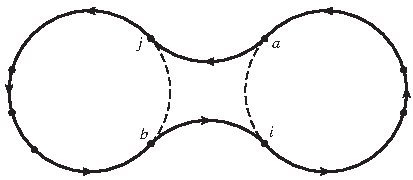
\includegraphics[width=0.567\linewidth,height=.8\textheight,keepaspectratio]{assets/p099_11.pdf}\end{center}
\begin{center}\small\textbf{8.20 Figure}\end{center}
\end{BookFloat}

Computing the product of the first three cycles in \BookInline{\tau \sigma = (i,\allowbreak j)\sigma,\allowbreak } we obtain

\begin{center}\begin{adjustbox}{max width=\linewidth}\BookInline{\displaystyle (i,\allowbreak j)(b,\allowbreak j,\allowbreak \times ,\allowbreak \times ,\allowbreak \times )(a,\allowbreak i,\allowbreak \times ,\allowbreak \times )= (a,\allowbreak j,\allowbreak \times ,\allowbreak \times ,\allowbreak \times ,\allowbreak b,\allowbreak i,\allowbreak \times ,\allowbreak \times ).}\end{adjustbox}\end{center}

The original 2 orbits have been joined to form just one in \BookInline{\tau \sigma } as symbolized in Fig. 8.20. Exercise 42 asks us to repeat the computation to show that the same thing happens if either one or both of \BookInline{i} and \BookInline{j} should be the only element of their orbit in \BookInline{\sigma.}

\noindent \textbf{Case II} Suppose \BookInline{i} and \BookInline{j} are in the same orbit of \BookInline{\sigma.} We can then write \BookInline{\sigma } as a product of disjoint cycles with the first cycle of the form

\begin{center}\begin{adjustbox}{max width=\linewidth}\BookInline{\displaystyle (a,\allowbreak i,\allowbreak \times ,\allowbreak \times ,\allowbreak \times ,\allowbreak b,\allowbreak j,\allowbreak \times ,\allowbreak \times )}\end{adjustbox}\end{center}

\end{BookBody}

% Source PDF page 100; original printed page 83
\BookSource{100}{83}
\BookNarrativetrue

\begin{BookBody}

shown symbolically by the circle in Fig. 8.20. Computing the product of the first two cycles in \BookInline{\tau \sigma = (i,\allowbreak j)\sigma,\allowbreak } we obtain

\begin{BookFloat}{08_groups_of_permutations-p100-1}
\begin{center}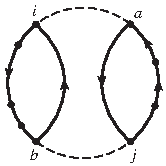
\includegraphics[width=0.228\linewidth,height=.8\textheight,keepaspectratio]{assets/p100_00.pdf}\end{center}
\begin{center}\small\textbf{8.21 Figure}\end{center}
\end{BookFloat}

\begin{center}\begin{adjustbox}{max width=\linewidth}\BookInline{\displaystyle (i,\allowbreak j)(a,\allowbreak i,\allowbreak \times ,\allowbreak \times ,\allowbreak \times ,\allowbreak b,\allowbreak j,\allowbreak \times ,\allowbreak \times )= (a,\allowbreak j,\allowbreak \times ,\allowbreak \times )(b,\allowbreak i,\allowbreak \times ,\allowbreak \times ,\allowbreak \times ).}\end{adjustbox}\end{center}

The original single orbit has been split into two as symbolized in Fig. 8.21.

We have shown that the number of orbits of \BookInline{\tau \sigma } differs from the number of orbits of \BookInline{\sigma } by 1. The identity permutation \BookInline{\iota } has \BookInline{n} orbits, because each element is the only member of its orbit. Now the number of orbits of a given permutation \BookInline{\sigma \in S_{n}} differs from \BookInline{n} by either an even or an odd number, but not both. Thus it is impossible to write

\begin{center}\begin{adjustbox}{max width=\linewidth}\BookInline{\displaystyle \sigma = \tau _{1}\tau _{2}\tau _{3}\cdots \tau _{m}\iota}\end{adjustbox}\end{center}

where the \BookInline{\tau _{k}} are transpositions in two ways, once with \BookInline{m} even and once with \BookInline{m} odd\BookInline{.}\BookEnd{\blacklozenge}

\BookLabel{8.22 Definition} A permutation of a finite set is\textbf{ even} or\textbf{ odd} according to whether it can be expressed as a product of an even number of transpositions or the product of an odd number of transpositions, respectively\BookInline{.}\BookEnd{\blacksquare}

\BookLabel{8.23 Example} The identity permutation \BookInline{\iota } in \BookInline{S_{n}} is an even permutation since we have \BookInline{\iota = (1,\allowbreak 2)(1,\allowbreak 2).} If \BookInline{n= 1} so that we cannot form this product, we define \BookInline{\iota } to be even. On the other hand, the permutation (1, 4, 5, 6) (2, 1, 5) in \BookInline{S_{6}} can be written as

\begin{center}\begin{adjustbox}{max width=\linewidth}\BookInline{\displaystyle (1,\allowbreak 4,\allowbreak 5,\allowbreak 6)(2,\allowbreak 1,\allowbreak 5)= (1,\allowbreak 6)(1,\allowbreak 5)(1,\allowbreak 4)(2,\allowbreak 5)(2,\allowbreak 1)}\end{adjustbox}\end{center}

\noindent which has five transpositions, so this is an odd permutation. \BookEnd{\blacktriangle}

\BookTextHeading{\textbf{The Alternating Groups}  }

\noindent We claim that for \BookInline{n\geq 2,\allowbreak } the number of even permutations in \BookInline{S_{n}} is the same as the number of odd permutations; that is\BookInline{,\allowbreak S_{n}} is split equally and both numbers are \BookInline{(n!)/2.} To show this, let \BookInline{A_{n}} be the set of even permutations in \BookInline{S_{n}} and let \BookInline{B_{n}} be the set of odd permutations for \BookInline{n\geq 2.} We proceed to define a one-to-one function from \BookInline{A_{n}} onto \BookInline{B_{n}.} This is exactly what is needed to show that \BookInline{A_{n}} and \BookInline{B_{n}} have the same number of elements.

Let \BookInline{\tau } be any fixed transposition in \BookInline{S_{n};} it exists since \BookInline{n\geq 2.} We may as well suppose that \BookInline{\tau = (1,\allowbreak 2).} We define a function

\begin{center}\begin{adjustbox}{max width=\linewidth}\BookInline{\displaystyle \lambda _{\tau }:A_{n}\to B_{n}}\end{adjustbox}\end{center}

\noindent by

\begin{center}\begin{adjustbox}{max width=\linewidth}\BookInline{\displaystyle \lambda _{\tau }(\sigma )= \tau \sigma ,\allowbreak }\end{adjustbox}\end{center}

\noindent that is\BookInline{,\allowbreak \sigma \in A_{n}} is mapped into \BookInline{(1,\allowbreak 2)\sigma } by \BookInline{\lambda _{\tau }.} Observe that since \BookInline{\sigma } is even, the permutation \BookInline{(1,\allowbreak 2)\sigma } can be expressed as a product of a \BookInline{(1+ } even number), or odd number, of transpositions, so \BookInline{(1,\allowbreak 2)\sigma } is indeed in \BookInline{B_{n}.} If for \BookInline{\sigma } and \BookInline{\mu } in \BookInline{A_{n}} it is true that \BookInline{\lambda _{\tau }(\sigma )= \lambda _{\tau }(\mu ),\allowbreak } then

\begin{center}\begin{adjustbox}{max width=\linewidth}\BookInline{\displaystyle (1,\allowbreak 2)\sigma = (1,\allowbreak 2)\mu ,\allowbreak }\end{adjustbox}\end{center}

\noindent and since \BookInline{S_{n}} is a group, we have \BookInline{\sigma = \mu.} Thus \BookInline{\lambda _{\tau }} is a one-to-one function. Finally,

\begin{center}\begin{adjustbox}{max width=\linewidth}\BookInline{\displaystyle \tau = (1,\allowbreak 2)= \tau ^{- 1},\allowbreak }\end{adjustbox}\end{center}

\noindent so if \BookInline{\rho \in B_{n},\allowbreak } then

\begin{center}\begin{adjustbox}{max width=\linewidth}\BookInline{\displaystyle \tau ^{- 1}\rho \in A_{n},\allowbreak }\end{adjustbox}\end{center}

\end{BookBody}

% Source PDF page 101; original printed page 84
\BookSource{101}{84}
\BookNarrativetrue

\begin{BookBody}

\noindent and

\begin{center}\begin{adjustbox}{max width=\linewidth}\BookInline{\displaystyle \lambda _{\tau }(\tau ^{- 1}\rho )= \tau (\tau ^{- 1}\rho )= \rho .}\end{adjustbox}\end{center}

\noindent Thus \BookInline{\lambda _{\tau }} maps onto \BookInline{B_{n}.} Hence the number of elements in \BookInline{A_{n}} is the same as the number in \BookInline{B_{n}} since there is a one-to-one correspondence between the elements of the sets.

Note that the product of two even permutations is again even. Also since \BookInline{n\geq 2,\allowbreak S_{n}} has the transposition (1, 2) and \BookInline{\iota = (1,\allowbreak 2)(1,\allowbreak 2)} is an even permutation. Finally, note that if \BookInline{\sigma } is expressed as a product of transpositions, the product of the same transpositions taken in just the opposite order is \BookInline{\sigma ^{- 1}.} Thus if \BookInline{\sigma } is an even permutation\BookInline{,\allowbreak \sigma ^{- 1}} must also be even. Referring to Theorem 5.12, we see that we have proved the following statement.

\BookLabel{8.24 Theorem} If \BookInline{n\geq 2,\allowbreak } then the collection of all even permutations of \BookInline{\{1,\allowbreak 2,\allowbreak 3,\allowbreak \cdots,\allowbreak n\}} forms a subgroup of order \BookInline{n!/2} of the symmetric group \BookInline{S_{n}.}

We can define a function called the\textbf{ sign of a permutation}, sgn \BookInline{:S_{n}\to \{1,\allowbreak - 1\}} by the formula

\begin{center}\begin{adjustbox}{max width=\linewidth}\BookInline{\displaystyle \operatorname { s g n } ( \sigma ) = \left\{ { \begin{array} { r l } { 1 \quad { \mathrm { i f ~ } } \sigma { \mathrm { ~ i s ~ e v e n } } } \\ { - 1 \quad { \mathrm { i f ~ } } \sigma { \mathrm { ~ i s ~ o d d } } . } \end{array} } \right.}\end{adjustbox}\end{center}

\noindent Thinking of \BookInline{\{1,\allowbreak - 1\}} as a group under multiplication, it is easy to see that sgn is a homomorphism. Since 1 is the identity in the group \BookInline{\{1,\allowbreak - 1\},\allowbreak } Ker(sgn\BookInline{)\; = } sgn\BookInline{- 1[\{1\}]} is a subgroup of \BookInline{S_{n}} consisting of all the even permutations. The homomorphism sgn is used in the standard way of defining the determinant of a square matrix. Exercise 52 asks you to prove some of the standard facts about determinants using this definition.

\BookLabel{8.25 Definition} The subgroup of \BookInline{S_{n}} consisting of the even permutations of \BookInline{n} letters is the\textbf{ alternating} \textbf{group} \BookInline{A_{n}} \textbf{on} \BookInline{n} \textbf{letters}\BookInline{.}\BookEnd{\blacksquare}

\noindent Both \BookInline{S_{n}} and \BookInline{A_{n}} are very important groups. Cayley’s theorem shows that every finite group \BookInline{G} is structurally identical to some subgroup of \BookInline{S_{n}} for \BookInline{n= |G|.} It can be shown that there are no formulas involving just radicals for solution of polynomial equations of degree \BookInline{n} for \BookInline{n\geq 5.} This fact is actually due to the structure of \BookInline{A_{n},\allowbreak } surprising as that may seem!

\end{BookBody}

\BookNarrativefalse

\begin{BookBody}

\BookExerciseTitle{8}

\BookTextHeading{\textbf{Computations}}

\noindent In Exercises 1 through 10 determine whether the given map is a group homomorphism. [Hint: To verify that a map is a homomorphism, you must check the homomorphism property. To check that a map is not a homomorphism you could either find \BookInline{a} and \BookInline{b} such that \BookInline{\phi (ab)\neq \phi (a)\phi (b),\allowbreak } or else you could determine that any of the properties in Theorem 8.5 fail.]

\BookExercise{1.}{Let \BookInline{\phi:\mathbb{Z}_{10}\to \mathbb{Z}_{2}} be given by \BookInline{\phi (x)= } the remainder when \BookInline{x} is divided by 2.}

\BookExercise{2.}{Let \BookInline{\phi:\mathbb{Z}_{9}\to \mathbb{Z}_{2}} be given by \BookInline{\phi (x)= } the remainder when \BookInline{x} is divided by 2.}

\BookExercise{3.}{Let \BookInline{\phi:\mathbb{Q}^{\ast }\to \mathbb{Q}^{\ast }} be given by \BookInline{\phi (x)= |x|.}}

\BookExercise{4.}{Let \BookInline{\phi:\mathbb{R}\to \mathbb{R}^{+ }} be given by \BookInline{\phi (x)= 2^{x}.}}

\BookExercise{5.}{Let \BookInline{\phi:D_{4}\to \mathbb{Z}_{4}} be given by \BookInline{\phi (\rho ^{i})= \phi (\mu \rho ^{i})= i} for \BookInline{0\leq i\leq 3.}}

\end{BookBody}

% Source PDF page 102; original printed page 85
\BookSource{102}{85}
\BookNarrativefalse

\begin{BookBody}

\BookExercise{6.}{Let \BookInline{F} be the additive group of all functions mapping \BookInline{\mathbb{R}} to \BookInline{\mathbb{R}.} Let \BookInline{\phi:F\to F} be given by \BookInline{\phi (f)= g} where \BookInline{g(x)= f(x)+ x.}}

\BookExercise{7.}{Let \BookInline{F} be as in Exercise 6 and \BookInline{\phi:F\to F} be defined by \BookInline{\phi (f)= 5f.}}

\BookExercise{8.}{\BookInline{\int _{0}^{1}g(x)dx.} Let \BookInline{F} be the additive group of all continuous functions mapping \BookInline{\mathbb{R}} to \BookInline{\mathbb{R}.} Let \BookInline{\phi:F\to \mathbb{R}} be defined by \BookInline{\phi (g)= }}

\BookExercise{9.}{Let \BookInline{M_{n}} be the additive group of \BookInline{n\times n} matrices with real entries. Let \BookInline{\phi:M_{n}\to \mathbb{R}} be given by \BookInline{\phi (A)= } det\BookInline{(A),\allowbreak } the determinant of \BookInline{A.}}

\BookExercise{10.}{Let \BookInline{M_{n}} be as in Exercise 9 and \BookInline{\phi:M_{n}\to \mathbb{R}} be defined by \BookInline{\phi (A)= } tr\BookInline{(A)} where tr\BookInline{(A)} is the trace of \BookInline{A,\allowbreak } which is the sum of the entries on the diagonal.}

\noindent In Exercises 11 through 16, compute the kernel for the given homomorphism \BookInline{\phi.}

\BookExercise{11.}{\BookInline{\phi:\mathbb{Z}\to \mathbb{Z}_{8}} such that \BookInline{\phi (1)= 6.}}

\BookExercise{12.}{\BookInline{\phi:\mathbb{Z}\to \mathbb{Z}} such that \BookInline{\phi (1)= 12.}}

\BookExercise{13.}{\BookInline{\phi:\mathbb{Z}\times \mathbb{Z}\to \mathbb{Z}} where \BookInline{\phi (1,\allowbreak 0)= 3} and \BookInline{\phi (0,\allowbreak 1)= - 5.}}

\BookExercise{14.}{\BookInline{\phi:\mathbb{Z}\times \mathbb{Z}\to \mathbb{Z}} where \BookInline{\phi (1,\allowbreak 0)= 6} and \BookInline{\phi (0,\allowbreak 1)= 9.}}

\BookExercise{15.}{\BookInline{\phi:\mathbb{Z}\times \mathbb{Z}\to \mathbb{Z}\times \mathbb{Z}} where \BookInline{\phi (1,\allowbreak 0)= (2,\allowbreak 5)} and \BookInline{\phi (0,\allowbreak 1)= (- 3,\allowbreak 2).}}

\BookExercise{16.}{Let \BookInline{D} be the additive group of all differentiable functions mapping \BookInline{\mathbb{R}} to \BookInline{\mathbb{R}} and \BookInline{F} the additive group of all functions from \BookInline{\mathbb{R}} to \BookInline{\mathbb{R}.\phi:D\to F} is given by \BookInline{\phi (f)= f^{\prime },\allowbreak } the derivative of \BookInline{f.}}

\noindent In Exercises 17 through 22, find all orbits of the given permutation.

\begin{enumerate}[start=17,label=\textbf{\arabic*.},leftmargin=2.5em,labelwidth=2em,labelsep=.5em,align=left]
\item \BookInline{\begin{pmatrix}1&2&3&4&5&6\\5&1&3&6&2&4\end{pmatrix}}
\item \BookInline{\begin{pmatrix}1&2&3&4&5&6&7&8\\5&6&2&4&8&3&1&7\end{pmatrix}}
\item \BookInline{\begin{pmatrix}1&2&3&4&5&6&7&8\\2&3&5&1&4&6&8&7\end{pmatrix}}
\item \BookInline{\sigma:\mathbb{Z}\to\mathbb{Z}} where \BookInline{\sigma(n)=n+1}.
\item \BookInline{\sigma:\mathbb{Z}\to\mathbb{Z}} where \BookInline{\sigma(n)=n+2}.
\item \BookInline{\sigma:\mathbb{Z}\to\mathbb{Z}} where \BookInline{\sigma(n)=n-3}.
\end{enumerate}
In Exercises 23 through 25, express the permutation of \BookInline{\{1,2,3,4,5,6,7,8\}} as a product of disjoint cycles, and then as a product of transpositions.
\begin{enumerate}[start=23,label=\textbf{\arabic*.},leftmargin=2.5em,labelwidth=2em,labelsep=.5em,align=left]
\item \BookInline{\begin{pmatrix}1&2&3&4&5&6&7&8\\8&2&6&3&7&4&5&1\end{pmatrix}}
\item \BookInline{\begin{pmatrix}1&2&3&4&5&6&7&8\\3&6&4&1&8&2&5&7\end{pmatrix}}
\item \BookInline{\begin{pmatrix}1&2&3&4&5&6&7&8\\5&3&2&8&4&7&6&1\end{pmatrix}}
\end{enumerate}

\BookExercise{26.}{Figure 8.26 shows a Cayley digraph for the alternating group \BookInline{A_{4}} using the generating set \BookInline{S= \{(1,\allowbreak 2,\allowbreak 3),\allowbreak } \BookInline{(1,\allowbreak 2)(3,\allowbreak 4)\}.} Continue labeling the other nine vertices with the elements of \BookInline{A_{4},\allowbreak } expressed as a product of disjoint cycles.}

\BookTextHeading{\textbf{Concepts}}

\noindent In Exercises 27 through 29, correct the definition of the italicized term without reference to the text, if correction is needed, so that it is in a form acceptable for publication.

\BookExercise{27.}{For a permutation \BookInline{\sigma } of a set \BookInline{A,\allowbreak } an\textit{ orbit} of \BookInline{\sigma } is a nonempty minimal subset of \BookInline{A} that is mapped onto itself by \BookInline{\sigma.}}

\BookExercise{28.}{The left regular representation of a group \BookInline{G} is the map of \BookInline{G} into \BookInline{S_{G}} whose value at \BookInline{g\in G} is the permutation of \BookInline{G} that carries each \BookInline{x\in G} into \BookInline{gx.}}

\BookExercise{29.}{The\textit{ alternating group} is the group of all even permutations.}

\end{BookBody}

% Source PDF page 103; original printed page 86
\BookSource{103}{86}
\BookNarrativefalse

\begin{BookBody}

\begin{BookFloat}{08_groups_of_permutations-p103-0}
\begin{center}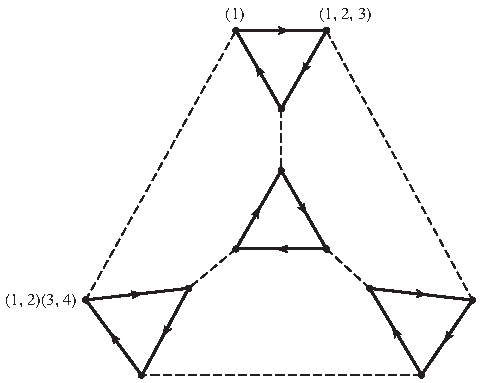
\includegraphics[width=0.658\linewidth,height=.8\textheight,keepaspectratio]{assets/p103_00.pdf}\end{center}
\begin{center}\small\textbf{8.26 Figure}\end{center}
\end{BookFloat}

\BookExercise{30.}{Before the proof of Cayley’s Theorem, it is shown that \BookInline{\lambda _{x}} is one-to-one. In the proof, one-to-one is shown again. Is it necessary to show one-to-one twice? Explain.}

\BookExercise{31.}{Determine whether each of the following is true or false.}

\BookExercise{a.}{Every permutation is a cycle.}

\BookExercise{b.}{Every cycle is a permutation.}

\BookExercise{c.}{The definition of even and odd permutations could have been given equally well before Theorem 8.19.}

\BookExercise{d.}{Every nontrivial subgroup \BookInline{H} of \BookInline{S_{9}} containing some odd permutation contains a transposition.}

\BookExercise{e.}{\textbf{e}\BookInline{.A_{5}} has 120 elements.}

\BookExercise{f.}{\textbf{f}\BookInline{.S_{n}} is not cyclic for any \BookInline{n\geq 1.}}

\BookExercise{g.}{\textbf{g}\BookInline{.A_{3}} is a commutative group.}

\BookExercise{h.}{\textbf{h}\BookInline{.S_{7}} is isomorphic to the subgroup of all those elements of \BookInline{S_{8}} that leave the number 8 fixed.}

\BookExercise{i.}{\textbf{i}\BookInline{.S_{7}} is isomorphic to the subgroup of all those elements of \BookInline{S_{8}} that leave the number 5 fixed.}

\BookExercise{j.}{The odd permutations in \BookInline{S_{8}} form a subgroup of \BookInline{S_{8}.}}

\BookExercise{k.}{Every group \BookInline{G} is isomorphic with a subgroup of \BookInline{S_{G}.}}

\BookExercise{32.}{The dihedral group is defined to be permutations with certain properties. Use the usual notation involving \BookInline{\mu } and \BookInline{\rho } for elements in \BookInline{D_{n}.}}

\BookExercise{a.}{Identify which elements in \BookInline{D_{3}} are even. Do the even elements form a cyclic group?}

\BookExercise{b.}{Identify which of elements of \BookInline{D_{4}} are even. Do the even elements form a cyclic group?}

\BookExercise{c.}{For which values of \BookInline{n} do the even permutations of \BookInline{D_{n}} form a cyclic group?}

\BookLabel{\textit{Proof}} \textbf{ Synopsis}

\BookExercise{33.}{Give a two-sentence synopsis of the proof of Cayley’s Theorem.}

\BookExercise{34.}{Give a two-sentence synopsis of the proof of Theorem 8.19.}

\BookTextHeading{\textbf{Theory}}

\BookExercise{35.}{Suppose that \BookInline{\phi:G\to G^{\prime }} is a group homomorphism and \BookInline{a\in } Ker\BookInline{\phi.} Show that for any \BookInline{g\in G,\allowbreak gag^{- 1}\in } Ker\BookInline{\phi.}}

\BookExercise{36.}{Prove that a homomorphism \BookInline{\phi:G\to G^{\prime }} is one-to-one if and only if Ker\BookInline{(\phi )} is the trivial subgroup of \BookInline{G.}}

\BookExercise{37.}{Let \BookInline{\phi:G\to G^{\prime }} be a group homomorphism. Show that \BookInline{\phi (a)= \phi (b)} if and only if \BookInline{a^{- 1}b\in } Ker\BookInline{\phi.}}

\BookExercise{38.}{Use Exercise 37 to prove that if \BookInline{\phi:G\to G^{\prime }} is a group homomorphism mapping onto \BookInline{G^{\prime }} and \BookInline{G} is a finite group, then for any \BookInline{b,\allowbreak c\in G^{\prime },\allowbreak |\phi ^{- 1}[\{b\}]|= |\phi ^{- 1}[\{c\}]|.} Conclude that if \BookInline{|G|} is a prime number, then either \BookInline{\phi } is an isomorphism or else \BookInline{G^{\prime }} is the trivial group.}

\end{BookBody}

% Source PDF page 104; original printed page 87
\BookSource{104}{87}
\BookNarrativetrue

\begin{BookBody}

\BookExercise{39.}{Show that if \BookInline{\phi:G\to G^{\prime }} and \BookInline{\gamma:G^{\prime }\to G^{\prime \prime }} are group homomorphisms, then \BookInline{\gamma \circ \phi:G\to G^{\prime \prime }} is also a group homomorphism.}

\BookExercise{40.}{Let \BookInline{\phi:G\to G^{\prime }} be a group homomorphism. Show that \BookInline{\phi [G]} is abelian if and only if \BookInline{xyx^{- 1}y^{- 1}\in } Ker\BookInline{(\phi )} for all \BookInline{x,\allowbreak y\in G.}}

\BookExercise{41.}{Prove the following about \BookInline{S_{n}} if \BookInline{n\geq 3.}}

\BookExercise{a.}{Every permutation in \BookInline{S_{n}} can be written as a product of at most \BookInline{n- 1} transpositions.}

\BookExercise{b.}{Every permutation in \BookInline{S_{n}} that is not a cycle can be written as a product of at most \BookInline{n- 2} transpositions.}

\BookExercise{c.}{Every odd permutation in \BookInline{S_{n}} can be written as a product of \BookInline{2n+ 3} transpositions, and every even permutation as a product of \BookInline{2n+ 8} transpositions.}

\BookExercise{42.}{\textbf{. a} Draw a figure like Fig. 8.20 to illustrate that if \BookInline{i} and \BookInline{j} are in different orbits of \BookInline{\sigma } and \BookInline{\sigma (i)= i,\allowbreak } then the number of orbits of \BookInline{(i,\allowbreak j)\sigma } is one less than the number of orbits of \BookInline{\sigma.}}

\BookExercise{b.}{Repeat part (a) if \BookInline{\sigma (j)= j} also.}

\BookExercise{43.}{Show that for every subgroup \BookInline{H} of \BookInline{S_{n}} for \BookInline{n\geq 2,\allowbreak } either all the permutations in \BookInline{H} are even or exactly half of them are even.}

\BookExercise{44.}{Let \BookInline{\sigma } be a permutation of a set \BookInline{A.} We shall say “\BookInline{\sigma } \textbf{moves} \BookInline{a\in A}” if \BookInline{\sigma (a)\neq a.} If \BookInline{A} is a finite set, how many elements are moved by a cycle \BookInline{\sigma \in S_{A}} of length \BookInline{n}?}

\BookExercise{45.}{Let \BookInline{A} be an infinite set. Let \BookInline{H} be the set of all \BookInline{\sigma \in S_{A}} such that the number of elements moved by \BookInline{\sigma (}see Exercise 44) is finite. Show that \BookInline{H} is a subgroup of \BookInline{S_{A}.}}

\BookExercise{46.}{Let \BookInline{A} be an infinite set. Let \BookInline{K} be the set of all \BookInline{\sigma \in S_{A}} that move (see Exercise 44) at most 50 elements of \BookInline{A.} Is \BookInline{K} a subgroup of \BookInline{S_{A}}? Why?}

\BookExercise{47.}{Consider \BookInline{S_{n}} for a fixed \BookInline{n\geq 2} and let \BookInline{\sigma } be a fixed odd permutation. Show that every odd permutation in \BookInline{S_{n}} is a product of \BookInline{\sigma } and some permutation in \BookInline{A_{n}.}}

\BookExercise{48.}{Show that if \BookInline{\sigma } is a cycle of odd length, then \BookInline{\sigma ^{2}} is a cycle.}

\BookExercise{49.}{Following the line of thought opened by Exercise 48, complete the following with a condition involving \BookInline{n} and \BookInline{r} so that the resulting statement is a theorem:}

\noindent If \BookInline{\sigma } is a cycle of length \BookInline{n,\allowbreak } then \BookInline{\sigma ^{r}} is also a cycle if and only if \BookInline{...}

\BookExercise{50.}{Show that \BookInline{S_{n}} is generated by \BookInline{\{(1,\allowbreak 2),\allowbreak (1,\allowbreak 2,\allowbreak 3,\allowbreak \cdots,\allowbreak n)\}.[}\textit{Hint:} Show that as \BookInline{r} varies\BookInline{,\allowbreak (1,\allowbreak 2,\allowbreak 3,\allowbreak \cdots,\allowbreak n)^{r}(1,\allowbreak 2)} \BookInline{(1,\allowbreak 2,\allowbreak 3,\allowbreak \cdots,\allowbreak n)^{n- r}} gives all the transpositions \BookInline{(1,\allowbreak 2),\allowbreak (2,\allowbreak 3),\allowbreak (3,\allowbreak 4),\allowbreak \cdots,\allowbreak (n- 1,\allowbreak n),\allowbreak (n,\allowbreak 1).} Then show that any transposition is a product of some of these transpositions and use Theorem 8.15.]}

\BookExercise{51.}{Let \BookInline{\sigma \in S_{n}} and define a relation on \BookInline{\{1,\allowbreak 2,\allowbreak 3,\allowbreak...,\allowbreak n\}} by \BookInline{i\sim j} if and only if \BookInline{j= \sigma ^{k}(i)} for some \BookInline{k\in \mathbb{Z}.}}

\BookExercise{1.}{Prove that \BookInline{\sim } is an equivalence relation.}

\BookExercise{2.}{Prove that for any \BookInline{1\leq i\leq n,\allowbreak } the equivalence class of \BookInline{i} is the orbit of \BookInline{i.}}

\BookExercise{52.}{The usual definition for the determinant of an \BookInline{n\times n} matrix \BookInline{A= (a_{i,\allowbreak j})} is}

\begin{center}\begin{adjustbox}{max width=\linewidth}\BookInline{\displaystyle \;\text{det}\;(A)= _{\sigma }\sum _{\in S_{n}}\;\text{sgn}\;(\sigma )a_{1,\allowbreak \sigma (1)}a_{2,\allowbreak \sigma (2)}a_{3,\allowbreak \sigma (3)}\cdots a_{n,\allowbreak \sigma (n)}}\end{adjustbox}\end{center}

\noindent where sgn\BookInline{(\sigma )} is the sign of \BookInline{\sigma.} Using this definition, prove the following properties of determinants.

\BookExercise{a.}{If a row of matrix \BookInline{A} has all zero entries, then det\BookInline{(A)= 0.}}

\BookExercise{b.}{If two different rows of \BookInline{A} are switched to obtain \BookInline{B,\allowbreak } then det\BookInline{(B)= - } det\BookInline{(A).}}

\BookExercise{c.}{If \BookInline{r} times one row of \BookInline{A} is added to another row of \BookInline{A} to obtain a matrix \BookInline{B,\allowbreak } then det\BookInline{(A)= } det\BookInline{(B)}}

\BookExercise{d.}{If a row of \BookInline{A} is multiplied by \BookInline{r} to obtain the matrix \BookInline{B,\allowbreak } then det\BookInline{(B)= r} det\BookInline{(A).}}

\BookExercise{53.}{Prove that any finite group \BookInline{G} is isomorphic with a subgroup of GL\BookInline{(n,\allowbreak \mathbb{R})} for some \BookInline{n.[}Hint: For each \BookInline{\sigma \in S_{n},\allowbreak } find a matrix in GL\BookInline{(n,\allowbreak \mathbb{R})} that sends each basis vector \BookInline{e_{i}} to \BookInline{e_{\sigma (i)}.} Use this to show that \BookInline{S_{n}} is isomorphic with a subgroup of GL\BookInline{(n,\allowbreak \mathbb{R}).]}}

\BookExercise{54.}{Prove Cayley’s Theorem using the right regular representation rather than the left regular representation.}

\BookExercise{55.}{Let \BookInline{\sigma \in S_{n}.} An inversion is a pair \BookInline{(i,\allowbreak j)} such that \BookInline{i<j} and \BookInline{\sigma (i)>\sigma (j).} Prove Theorem 8.19 by showing that multiplying a permutation by a transposition changes the number of inversions by an odd number.}

\end{BookBody}

% Continuation on source PDF page 105, preceding Section 9
\BookNarrativefalse

\begin{BookBody}

\BookExercise{56.}{The sixteen puzzle consists of 15 tiles numbered 1 through 15 arranged in a four-by-four grid with one position left blank. A move is sliding a tile adjacent to the blank position into the blank position. The goal is to arrange the numbers in order by a sequence of moves. Is it possible to start with the configuration pictured in Figure 8.27(a) and solve the puzzle as indicated in Figure 8.27(b)? Prove your answer by finding a sequence of moves to solve the puzzle or by proving that it is impossible to solve.}

\begin{BookFloat}{08_groups_of_permutations-p105-1}
\begin{center}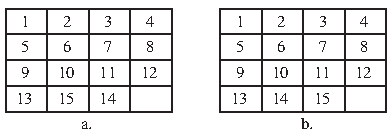
\includegraphics[width=0.536\linewidth,height=.8\textheight,keepaspectratio]{assets/p105_01.pdf}\end{center}
\begin{center}\small\textbf{8.27 Figure}\end{center}
\end{BookFloat}

\end{BookBody}
\ifdefined\BookMaster\let\BookFinish\relax\else\def\BookFinish{\end{document}}\fi\BookFinish
